\documentclass[11pt,letter]{exam}
\topmargin -0.15in \textheight 8.5in \textwidth 6.5in \oddsidemargin
0in \evensidemargin 0in
\usepackage{graphicx}
\usepackage{amsmath, amssymb}
\newcommand{\ben}{\begin{enumerate}}
\newcommand{\een}{\end{enumerate}}
\usepackage{amsfonts}

\usepackage{color}
\usepackage{graphicx}
\usepackage[latin1]{inputenc}
\usepackage{tikz}
\usetikzlibrary{trees}
\usepackage{verbatim}



\begin{document}

% Set the overall layout of the tree
\tikzstyle{level 1}=[level distance=3.5cm, sibling distance=2.5cm]
\tikzstyle{level 2}=[level distance=3.5cm, sibling distance=1.5cm]

% Define styles for bags and leafs
\tikzstyle{bag} = [text width=4em, text centered]
\tikzstyle{end} = [circle, minimum width=3pt,fill, inner sep=0pt]

\CorrectChoiceEmphasis{\color{red}\bfseries}
\bracketedpoints
\pointpoints{pt}{pts}
\setlength\answerskip{0.05ex}

\begin{center}
{\Large {\bf CMSE 381  MIDTERM} }
\end{center}
\vspace{1cm}

Feb 19, 2020 \hfill Time allowed: 70 minutes \vspace{1 cm}

{\bf Name: \underline {\hspace{2in}}} \hspace{1cm}

\vspace*{0.7in}

{\bf Pledge}: {\it I have neither given nor received any unauthorized aid during this exam.}
\vspace*{1.25cm}\\
Signature \rule{5cm}{.5mm}\vspace*{0.7in}

{\bf Instructions:}\\
\vspace*{.1in}
\\
For all the questions, show all your work in the space provided. You will NOT receive credit if you do not justify your answers. \\
\vspace*{.1in}\\
This is a closed book and closed notes examination.
\vspace*{.1in}\\
Please budget you time so that you have sufficient time to do all the  questions.


\mbox{}

\makebox[5.5in]{\hrulefill}\\



\vspace*{0.2in}
 {\bf Good luck!}
\newpage

%%%%%%%%Multiple Choice (30 Questions: 2 points a piece)%%%%%%%%%%%%%%

%%%%%%%%Multiple Choice (30 Questions: 2 points a piece)%%%%%%%%%%%%%%
\begin{questions}


\item (3 pts)   In a marketing setting, we have demographic information for a number of potential customers. We may wish to understand which types of customers are similar to each other by grouping individuals according to their observed characteristics. Is this a supervised or unsupervised learning? Explain your choice. 

\vspace{4 cm}

\item (5 pts) The following figure displays the average training and testing MSEs as a function of model flexibility. 
Explain the meaning of the three curves and justify your answer. \\
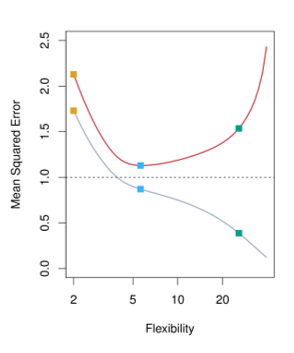
\includegraphics[width=5cm]{./Picture1.png}

\item (5 pts) We are trying to predict whether a patient will have a heart attach within one year. We have tried four different methods on a training dataset and have the following ROC curves
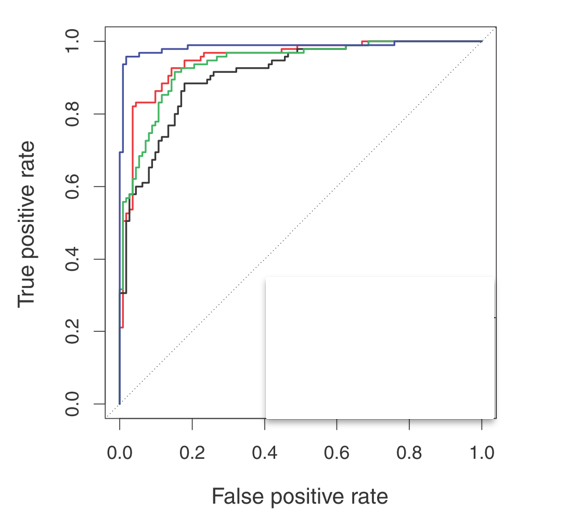
\includegraphics[width=5cm]{./Picture3.png}\\
Which curve has the best performance on this training set? Justify your answer.
\newpage
\item (7 pts) Assume the true model is 
\[ 
 Y = f(X) + \epsilon.
\]
We have a set of training data Tr, which is used to fit a model $\hat{f}(x)$, and a new testing data $(x_0, y_0)$. Here, we assume $x_0$ are fixed.
Derive 
\[
	   E \left[ \big( y_0 - \hat{f}(x_0) \big)^2 \right]  = Var(\hat{f}(x_0)) + [Bias( \hat{f}(x_0))]^2 + Var(\epsilon).
\]

\newpage

\item  We assume $Y = \beta_0 + \beta_1 X + \epsilon$, where $\epsilon \sim N(0, \sigma^2)$. We collect a set of i.i.d. training data $\{(x_1, y_1), \ldots, (x_n, y_n) \}$ and want to fit a linear regression.
	\begin{itemize}
	\item[a.] (5 pts) Derive the $\hat{\beta}_0$ and $\hat{\beta}_1$ which minimize the RSS.
	\item[b.] (5 pts) Let $\epsilon_i = y_i - \hat{\beta}_0 - \hat{\beta}_1 x_i$. Prove that $\sum_{i = 1}^n \epsilon_i x_i = 0$. 
	\item[c.] (5 pts) If $X$ is  the ethnicity variable including three levels $\{$Asian, African American, Caucasian    $\}$, how can we include it into the linear model?
	\end{itemize}
\newpage
	 \item We know to build a classification model with $Y \in \{0, 1 \}$  and $X \in \mathbb{R}^p$. We collect a set of i.i.d. training data $\{(x_1, y_1), \ldots, (x_n, y_n) \}$, where $x_i \in \mathbb{R}^p$. 
\begin{enumerate}
\item[a.] (3 pts)First, we want to fit a logistic regression model. Write down the logistic regression model. \\

\item[b.] (7 pts) As discussed in the class, we will use maximum likelihood framework to estimate the parameters in the logistic regress model. Write out the log likelihood of the training data.
\item[c.] (5 pts) Using logistic regression, we normally will classify a data as follows
\begin{equation} \notag
  Y =
    \begin{cases}
      1 & \text{if Pr$(Y = 1 | X = x) \geq 0.5$ }\\
      0 & \text{otherwise}.
    \end{cases}     
\end{equation}
Assuming we want to classify a patient into either HIV positive $(Y = 1)$ or HIV negative $(Y = 0)$. In this case, we have worse consequence to have a Type II error than Type I error. To address this, how will you modify the model above to predict $Y$ to reduce the type II error? Justify your answer.

\item[d.] (Extra 5 pts) When we use LDA to perform the classification, the classifier will be  
\begin{equation}  \notag
  Y =
    \begin{cases}
      1 & \text{if $\delta_1(x) \geq \delta_0(x)$ }\\
      0 & \text{otherwise}.
    \end{cases}     
\end{equation}
Prove that this is equivalent to the classifier in (c). Namely, when $\delta_1(x) \geq \delta_0(x)$, Pr$(Y = 1 | X = x) \geq 0.5$. Here, 
\[  
	\delta_k(x) = x^T \Sigma^{-1}\mu_k - \frac{1}{2} \mu_k^T \Sigma^{-1} \mu_k + \log \pi_k.
\] And if $X \sim N(\mu, \Sigma)$, then its probability density function for $X = x$ is 
\[
	f(x) = \frac{1}{(2\pi)^{p/2} |\Sigma|^{1/2}} e^{-\frac{1}{2}(x - \mu)^T \Sigma^{-1}(x - \mu) }
\]
\end{enumerate}
\newpage


\end{questions}


\end{document} } 